\documentclass[a4paper, 12pt]{report}

%====================== PACKAGES ======================

\usepackage[english]{babel}
\usepackage[utf8x]{inputenc}
%pour gérer les positionnement d'images
\usepackage{float}
\usepackage{amsmath}
\usepackage{graphicx}
\usepackage[colorinlistoftodos]{todonotes}
\usepackage{url}
%pour les informations sur un document compilé en PDF et les liens externes / internes
\usepackage{hyperref}
%pour la mise en page des tableaux
\usepackage{array}
\usepackage{tabularx}
%pour utiliser \floatbarrier
%\usepackage{placeins}
%\usepackage{floatrow}
%espacement entre les lignes
\usepackage{setspace}
%modifier la mise en page de l'abstract
\usepackage{abstract}
%police et mise en page (marges) du document
\usepackage[T1]{fontenc}
\usepackage[top=2cm, bottom=2cm, left=2cm, right=2cm]{geometry}
%Pour les galerie d'images
\usepackage{subfig}
\usepackage{eurosym}
%Pour la mise en page du code
\usepackage{listings}
\usepackage{color}
\definecolor{dkgreen}{rgb}{0,0.6,0}
\definecolor{gray}{rgb}{0.5,0.5,0.5}
\definecolor{mauve}{rgb}{0.58,0,0.82}
\definecolor{darkWhite}{rgb}{0.94,0.94,0.94}
\definecolor{black}{rgb}{0,0,0}




\lstdefinestyle{tf}{frame=shadowbox,
	rulesepcolor=\color{gray},
	framexleftmargin=5mm,
	aboveskip=3mm,
	belowskip=3mm,
	showstringspaces=false,
	columns=flexible,
	basicstyle={\small\ttfamily},
	numbers=left,
	numberstyle=\tiny,
	breaklines=true,
	tabsize=3
}

\lstdefinestyle{console}{frame=shadowbox,
	backgroundcolor=\color{darkWhite},
	rulesepcolor=\color{gray},
	framexleftmargin=5mm,
	aboveskip=3mm,
	belowskip=3mm,
	showstringspaces=false,
	columns=flexible,
	basicstyle={\small\ttfamily},
	numbers=left,
	numberstyle=\tiny,
	breaklines=true,
	tabsize=3
}

\lstdefinestyle{color}{
	otherkeywords={1, 2, 3, 4, 5, 6, 7, 8, 9, 0},
	keywordstyle=\color{blue},
	stringstyle=\color{mauve}
}


\lstset{frame=tb,
	extendedchars=true,
	inputencoding=latin1,
	rulesepcolor=\color{gray},
	framexleftmargin=5mm,
	aboveskip=3mm,
	belowskip=3mm,
	showstringspaces=false,
	columns=flexible,
	basicstyle={\small\ttfamily},
	numbers=left,
	numberstyle=\tiny,
	breaklines=true,
	tabsize=3,
	literate=%
	{é}{{\'e}}{1}%
	{è}{{\`e}}{1}%
	{à}{{\`a}}{1}%
	{ç}{{\c{c}}}{1}%
	{œ}{{\oe}}{1}%
	{ù}{{\`u}}{1}%
	{É}{{\'E}}{1}%
	{È}{{\`E}}{1}%
	{À}{{\`A}}{1}%
	{Ç}{{\c{C}}}{1}%
	{Œ}{{\OE}}{1}%
	{Ê}{{\^E}}{1}%
	{ê}{{\^e}}{1}%
	{î}{{\^i}}{1}%
	{ô}{{\^o}}{1}%
	{û}{{\^u}}{1}%
	{ä}{{\"{a}}}1
	{ë}{{\"{e}}}1
	{ï}{{\"{i}}}1
	{ö}{{\"{o}}}1
	{ü}{{\"{u}}}1
	{û}{{\^{u}}}1
	{â}{{\^{a}}}1
	{Â}{{\^{A}}}1
	{Î}{{\^{I}}}1
}

%====================== INFORMATION ET REGLES ======================

%rajouter les numérotation pour les \paragraphe et \subparagraphe
\setcounter{secnumdepth}{4}
\setcounter{tocdepth}{4}

\hypersetup{							% Information sur le document
pdfauthor = {Sugdenaz EKICI,
			Yahia KHERZA,
			Olivier MARAVAL,
    		Valentin VIRET-JACQUOT},			% Auteurs
pdftitle = {Architecture logicielle et notice d'installation / utilisation du poste de développement},			% Titre du document
pdfsubject = {Mémoire de Projet},		% Sujet
pdfkeywords = {Tag1, Tag2, Tag3, ...},	% Mots-clefs
pdfstartview={FitH}}					% ajuste la page à la largueur de l'écran
%pdfcreator = {MikTeX},% Logiciel qui a crée le document
%pdfproducer = {}} % Société avec produit le logiciel

%======================== DEBUT DU DOCUMENT ========================

\begin{document}

\addtocontents{toc}{\protect\thispagestyle{empty}}

%régler l'espacement entre les lignes
\newcommand{\HRule}{\rule{\linewidth}{0.5mm}}

%page de garde
\begin{titlepage}
\begin{center}

% Upper part of the page. The '~' is needed because only works if a paragraph has started.

\includegraphics[width=0.5\textwidth]{./images/InfoLogoQuadriH.png}~\\[1cm]

\textsc{\LARGE SAE 1.01-02 - BUT INFORMATIQUE - GROUPE 1 }\\[1.5cm]

\textsc{\Large }\\[0.5cm]

% Title
\HRule \\[0.4cm]

{\huge \bfseries Comparative Study of Two Low-Pass Filters for Sound Data Playback: Analysis and Performance\\[0.4cm] }

\HRule \\[1.5cm]

% Author and supervisor
\begin{minipage}{0.4\textwidth}
\begin{flushleft} \large
\emph{Auteur:}\\
Yahia \textsc{Kherza}(\textit{A1})\\
Olivier \textsc{Maraval}(\textit{A1})\\
\end{flushleft}
\end{minipage}
\begin{minipage}{0.4\textwidth}
\begin{flushright} \large
\emph{Client:} \\
Gilles \textsc{Perrot}\\
\emph{Référent:} \\
Olivier \textsc{Maraval}
\end{flushright}
\end{minipage}

\vfill

% Bottom of the page
{\large \today}

\end{center}
\end{titlepage}

%page blanche
\newpage
~
\thispagestyle{empty}

\pagenumbering{gobble}
\tableofcontents
\thispagestyle{empty}

%ne pas numéroter le sommaire

\newpage

%espacement entre les lignes d'un tableau
\renewcommand{\arraystretch}{1.5}

%====================== INCLUSION DES PARTIES ======================

~
\thispagestyle{empty}


\newpage
\pagenumbering{arabic}

\setcounter{page}{6}

\chapter{Introduction}

The objective is to examine and compare two low-pass filter designs with the end goal of enhancing the clarity of text data transmitted via audio signals. This comparison is a component of a larger project, the DosOok challenge, which involves the development of the two programs DosSend and DosRead for sending and receiving text data through sound.

In this context, a low-pass filter is crucial as it allows the desired signal to pass while attenuating frequencies that are not needed. The necessity for this comparison comes from the fact that we need to find the best speed to noise reduction ratio.

For this study, two distinct low-pass filtering techniques have been selected. The criteria for their evaluation are the speed of processing and their smoothing capability. The filter will get a pass if the initial text isn't altered after the signal has been processed.

This report will detail the theoretical concepts behind each filter, the process of their implementation in Java, and the outcomes of their performance tests. The aim is to determine which filter provides a superior solution for the problem at hand.
\chapter{Methodology}

We will create our sound containing the data in a text file with the DosSend program. We will then read it back with DosRead and see how fast we can get back the former data.

\section{DosSend and DosRead usage}

\subsection{Using DosSend to create a wav file}

\subsubsection{Compiling the Program}

Compile the Java code using a Java compiler

\begin{lstlisting}
javac DosSend.java StdDraw.java
\end{lstlisting}

\subsubsection{Run the Program}

Run the compiled classes with Java and send it your data written in a .txt file.

\begin{lstlisting}
java DosSend.java < textfile.txt
\end{lstlisting}

\subsubsection{Output}

The program will convert the input text into an audio signal and save it as \texttt{DosOok\_message.wav}. It will also print characteristics of the signal to the console and display a graphical representation of the signal waveform.

\begin{figure}[!h]
	\begin{lstlisting}[style=console]
	[oli@oli-arch src]$ java DosSend < helloWorld.txt
	[ H e l l o   W o r l d   ! ]
	[ 1 0 1 0 1 0 1 0 0 0 0 1 0 0 1 0 1 0 1 0 0 1 1 0 0 0 1 1 0 1 1 0 0 0 1 1 0 1 1 0 1 1 1 1 0 1 1 0 0 0 0 0 0 1 0 0 1 1 1 0 1 0 1 0 1 1 1 1 0 1 1 0 0 1 0 0 1 1 1 0 0 0 1 1 0 1 1 0 0 0 1 0 0 1 1 0 0 0 0 0 0 1 0 0 1 0 0 0 0 1 0 0 ]
	Message : Hello World !
	Nombre de symboles : 13
	Nombre d'échantillons : 49392
	Durée : 1.12 s
	\end{lstlisting}
	\caption{Console output for the text "Hello World !"}
\end{figure}

\begin{figure}[!h]
	\begin{center}
		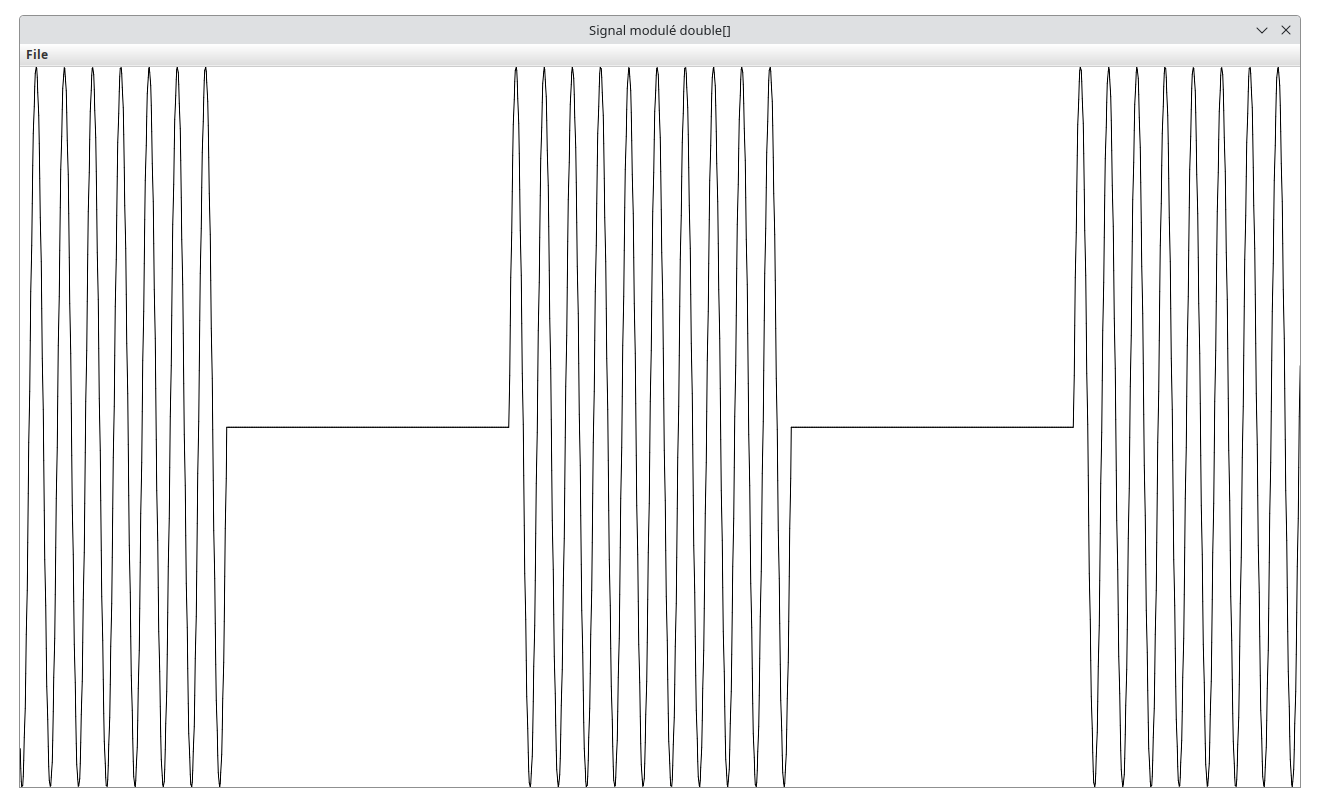
\includegraphics[width=15cm]{images/StdDraw1.png}
	\end{center}
	\caption{Signal output for the text "Hello World !" with start:300 stop:1000 mode:line}
\end{figure}

\subsection{Using DosRead}

\section{Monitoring the speed of the filter}

\section{Checking the filter's accuracy}
\chapter{Results}

\section{Speed}

\subsection{LPFilter's Speed to Filtering Strength}

\begin{table}[htbp]
	\centering
	\begin{tabularx}{\textwidth}{|X|X|X|}
		\hline
		\textbf{Cut Off Frequency Hz} & \textbf{SMA processing time (ms)} & \textbf{EMA processing time (ms)} \\ \hline
		\textbf{20} & 2788 & 947 \\ \hline
		\textbf{500} & 11980 & 972 \\ \hline
		\textbf{1000} & 26930 & 972 \\ \hline
	\end{tabularx}
	\caption{Processing Time Comparison}
\end{table}


\begin{figure}[!h]
	\begin{center}
		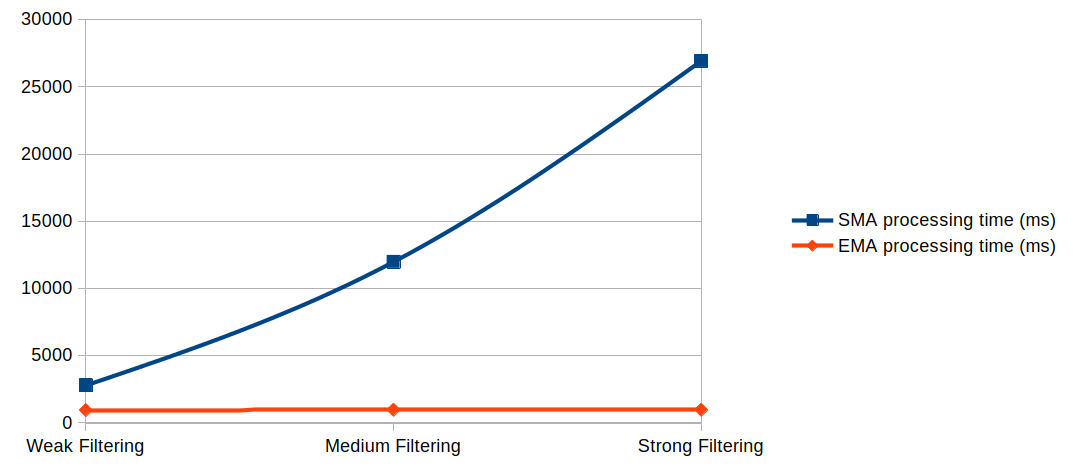
\includegraphics[width=15cm]{images/GraphSpeedtoFilteringStrength.png}
	\end{center}
	\caption{Processing speed of each filter as their cut off frequency decreases}
\end{figure}

\subsection{LPFilter's Speed to Data Length}

\begin{figure}[!h]
	\begin{center}
		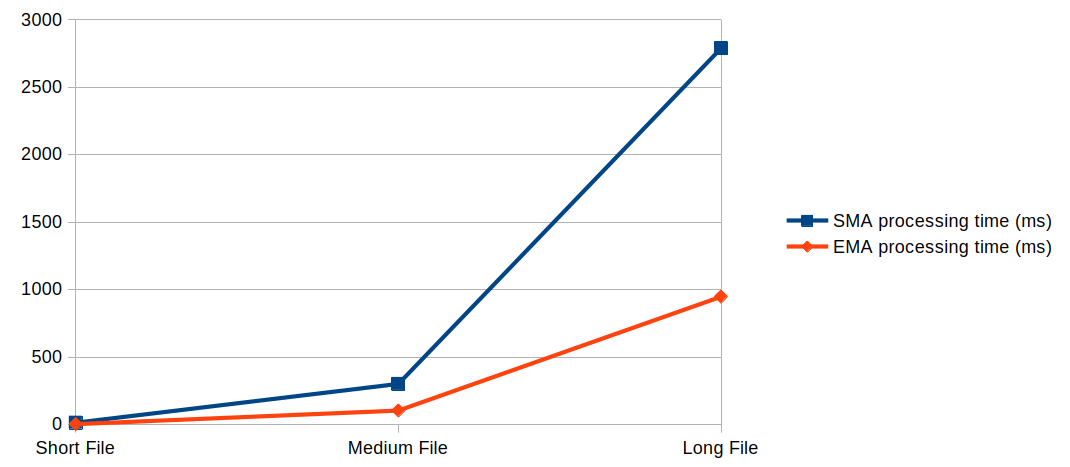
\includegraphics[width=15cm]{images/GraphSpeedtoLength.png}
	\end{center}
	\caption{Processing speed of each filters as the length of the data increases}
\end{figure}

\begin{table}[!h]
	\centering
	\begin{tabularx}{\textwidth}{|X|X|X|X|}
		\hline
		\textbf{File} & \textbf{Characters} & \textbf{SMA processing time (ms)} & \textbf{EMA processing time (ms)} \\ \hline
		\textbf{Short File} & \textbf{13} & 14 & 3 \\ \hline
		\textbf{Medium File} & \textbf{641} & 301 & 104 \\ \hline
		\textbf{Long File} & \textbf{6307} & 2788 & 947 \\ \hline
	\end{tabularx}
	\caption{Processing Time Comparison}
\end{table}

\subsection{LPFilter's Efficiency}

\begin{table}[!h]
	\centering
	\begin{tabularx}{\textwidth}{|X|X|X|X|}
		\hline
		\textbf{File} & \textbf{Characters} & \textbf{SMA processing time (ms)} & \textbf{EMA processing time (ms)} \\ \hline
		\textbf{Short File} & \textbf{13} & 14 & 3 \\ \hline
		\textbf{Medium File} & \textbf{641} & 301 & 104 \\ \hline
		\textbf{Long File} & \textbf{6307} & 2788 & 947 \\ \hline
	\end{tabularx}
	\caption{Processing Time Comparison}
\end{table}

\newpage

\subsection{LPFilter's Output}

\subsubsection{Filters Frequency Response and efficiency}

\begin{figure}[!h]
	\begin{center}
		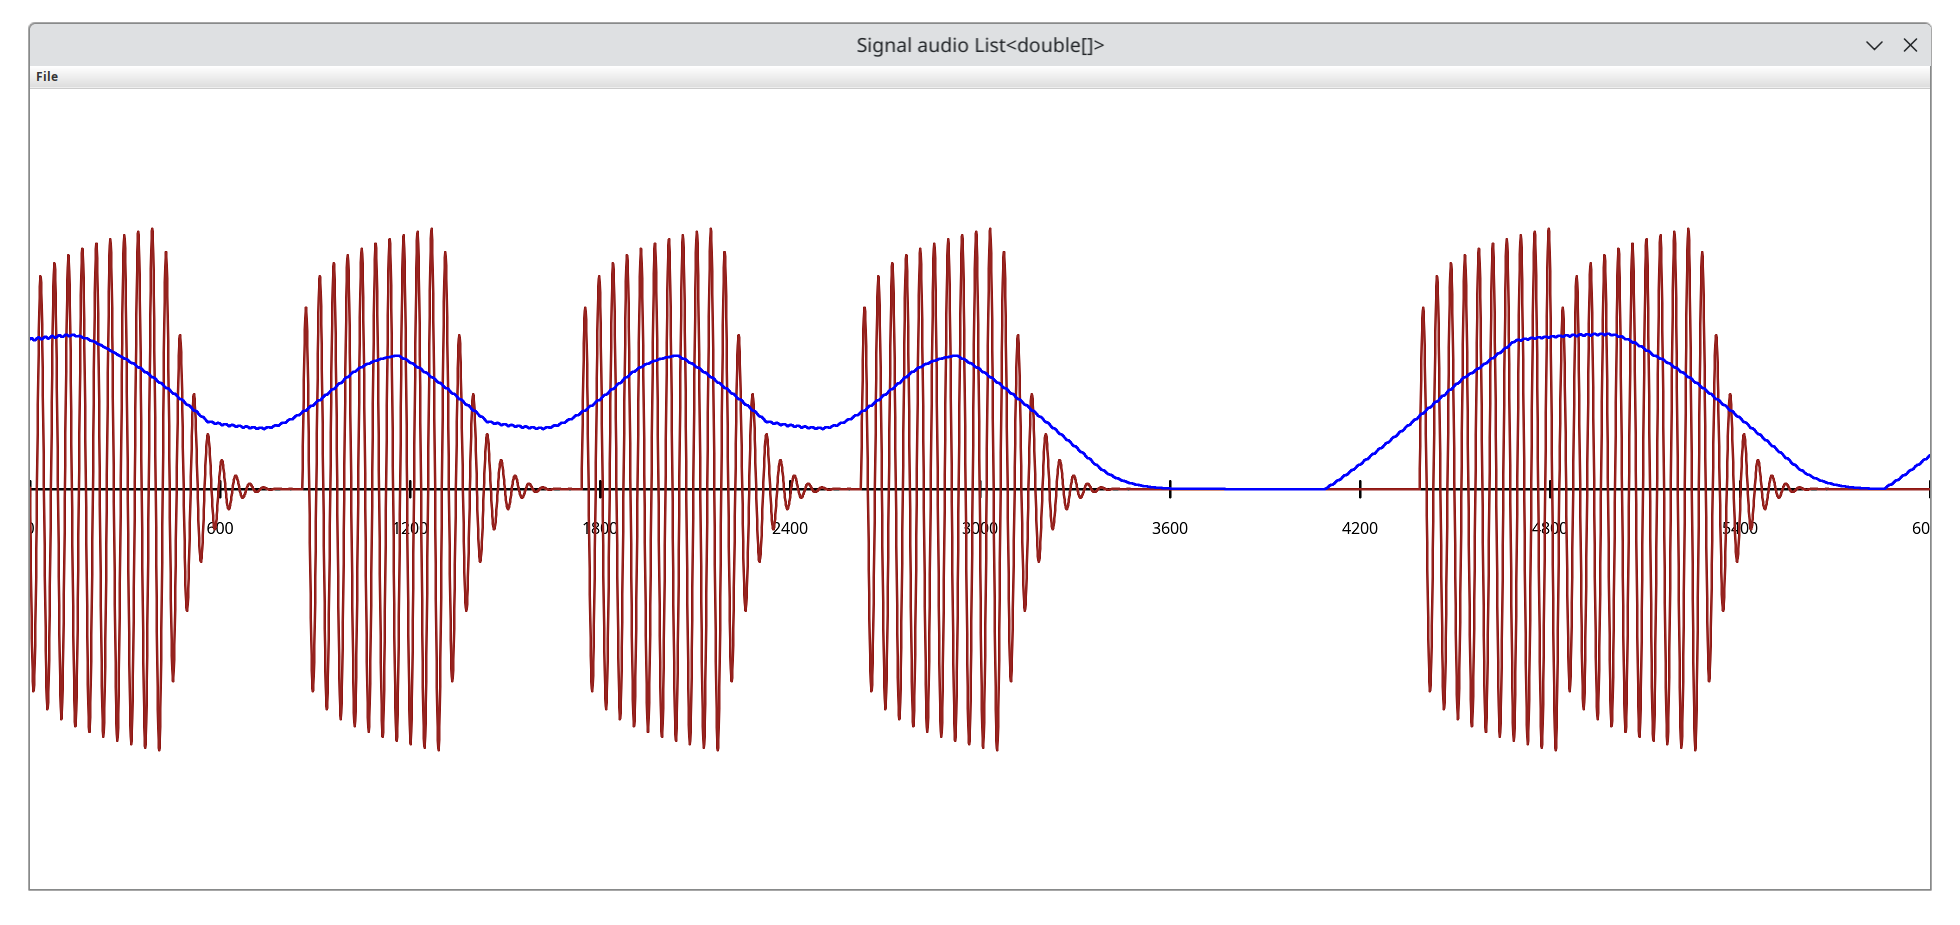
\includegraphics[width=15cm]{images/LP1600.png}
	\end{center}
	\caption{\textbf{SMA} Filter output in blue for a cut off frequency of \textbf{20Hz}}
\end{figure}

\begin{figure}[!h]
	\begin{center}
		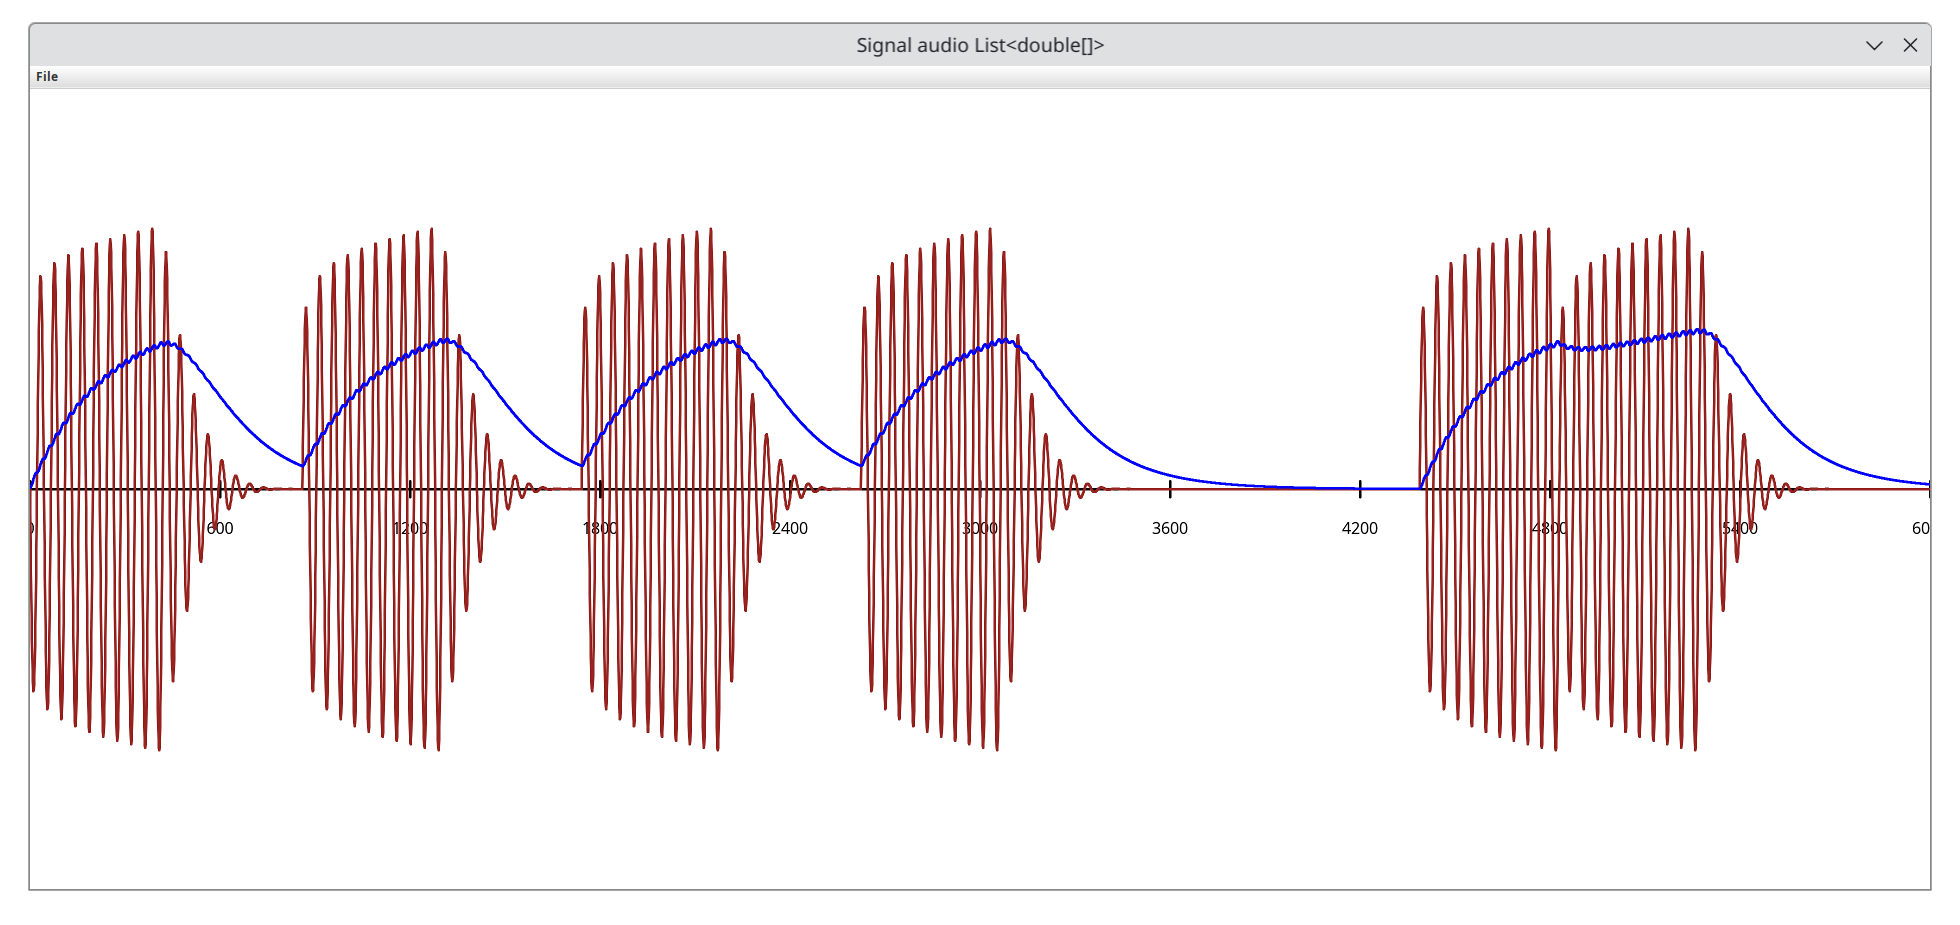
\includegraphics[width=15cm]{images/LP240.png}
	\end{center}
	\caption{\textbf{EMA} Filter output in blue for a cut off frequency of \textbf{20Hz}}
\end{figure}

\begin{figure}[!h]
	\begin{center}
		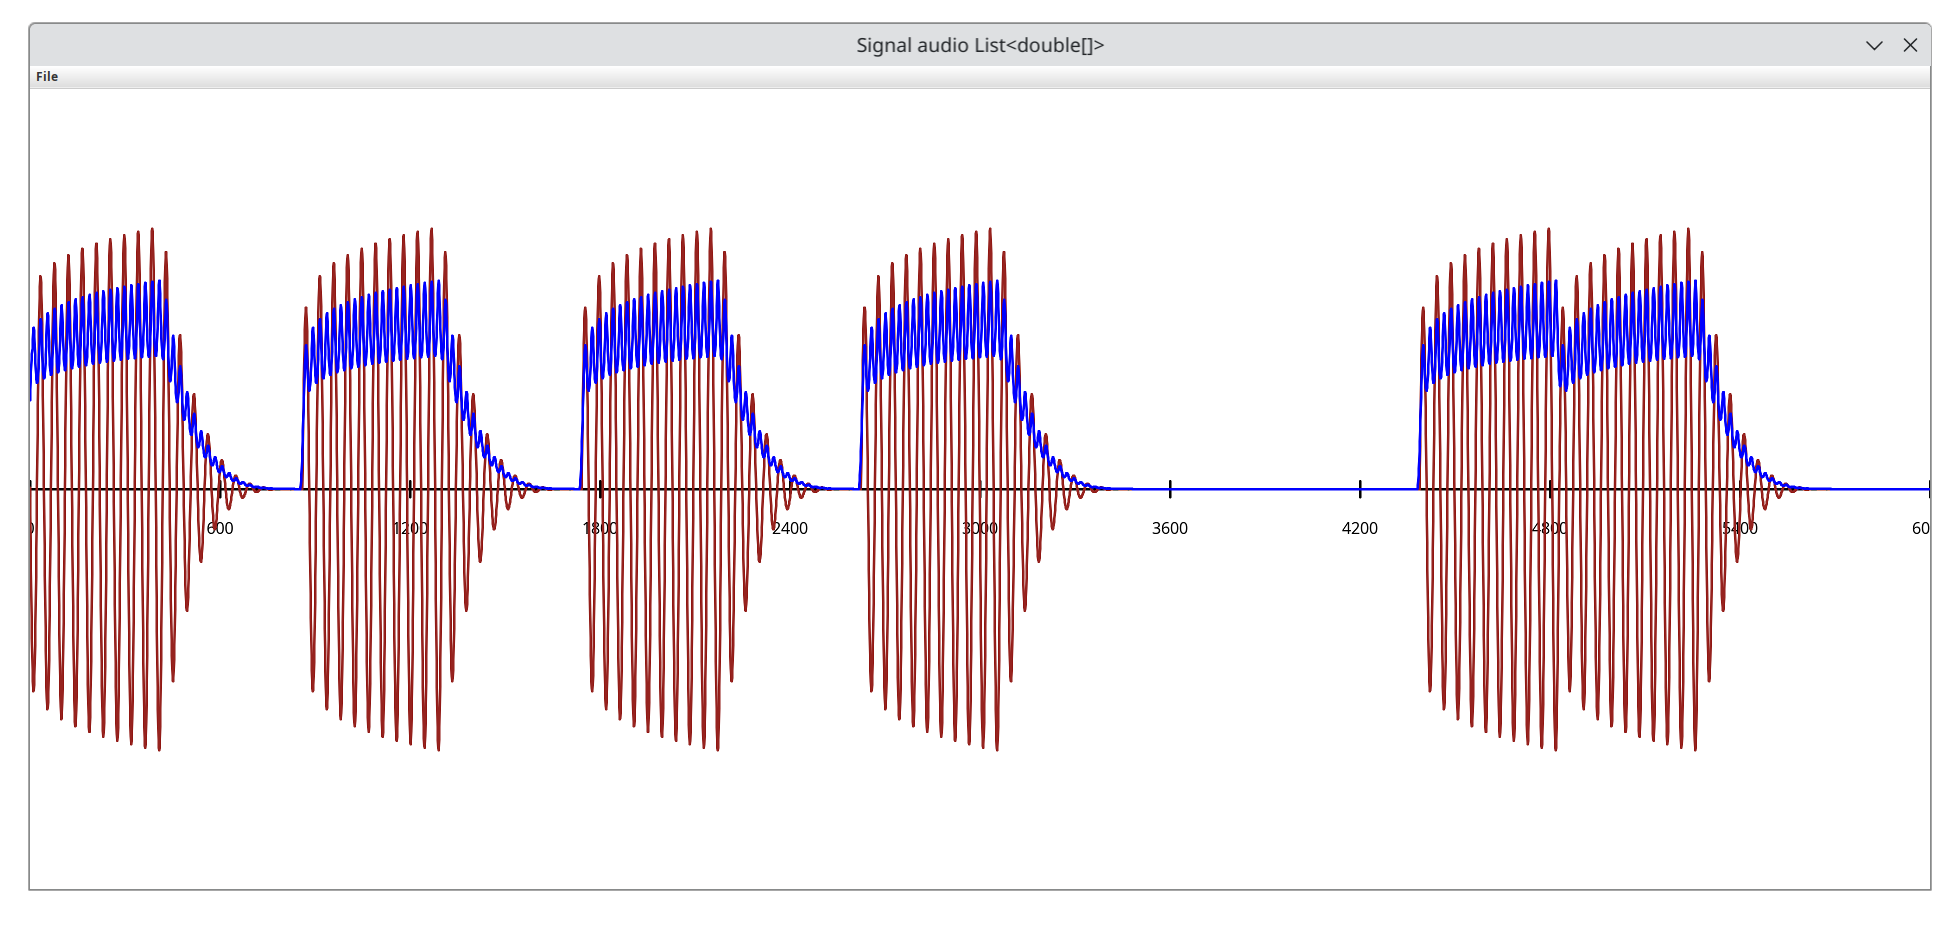
\includegraphics[width=15cm]{images/LP116.png}
	\end{center}
	\caption{\textbf{SMA} Filter output in blue for a cut off frequency of \textbf{1kHz}}
\end{figure}

\begin{figure}[!h]
	\begin{center}
		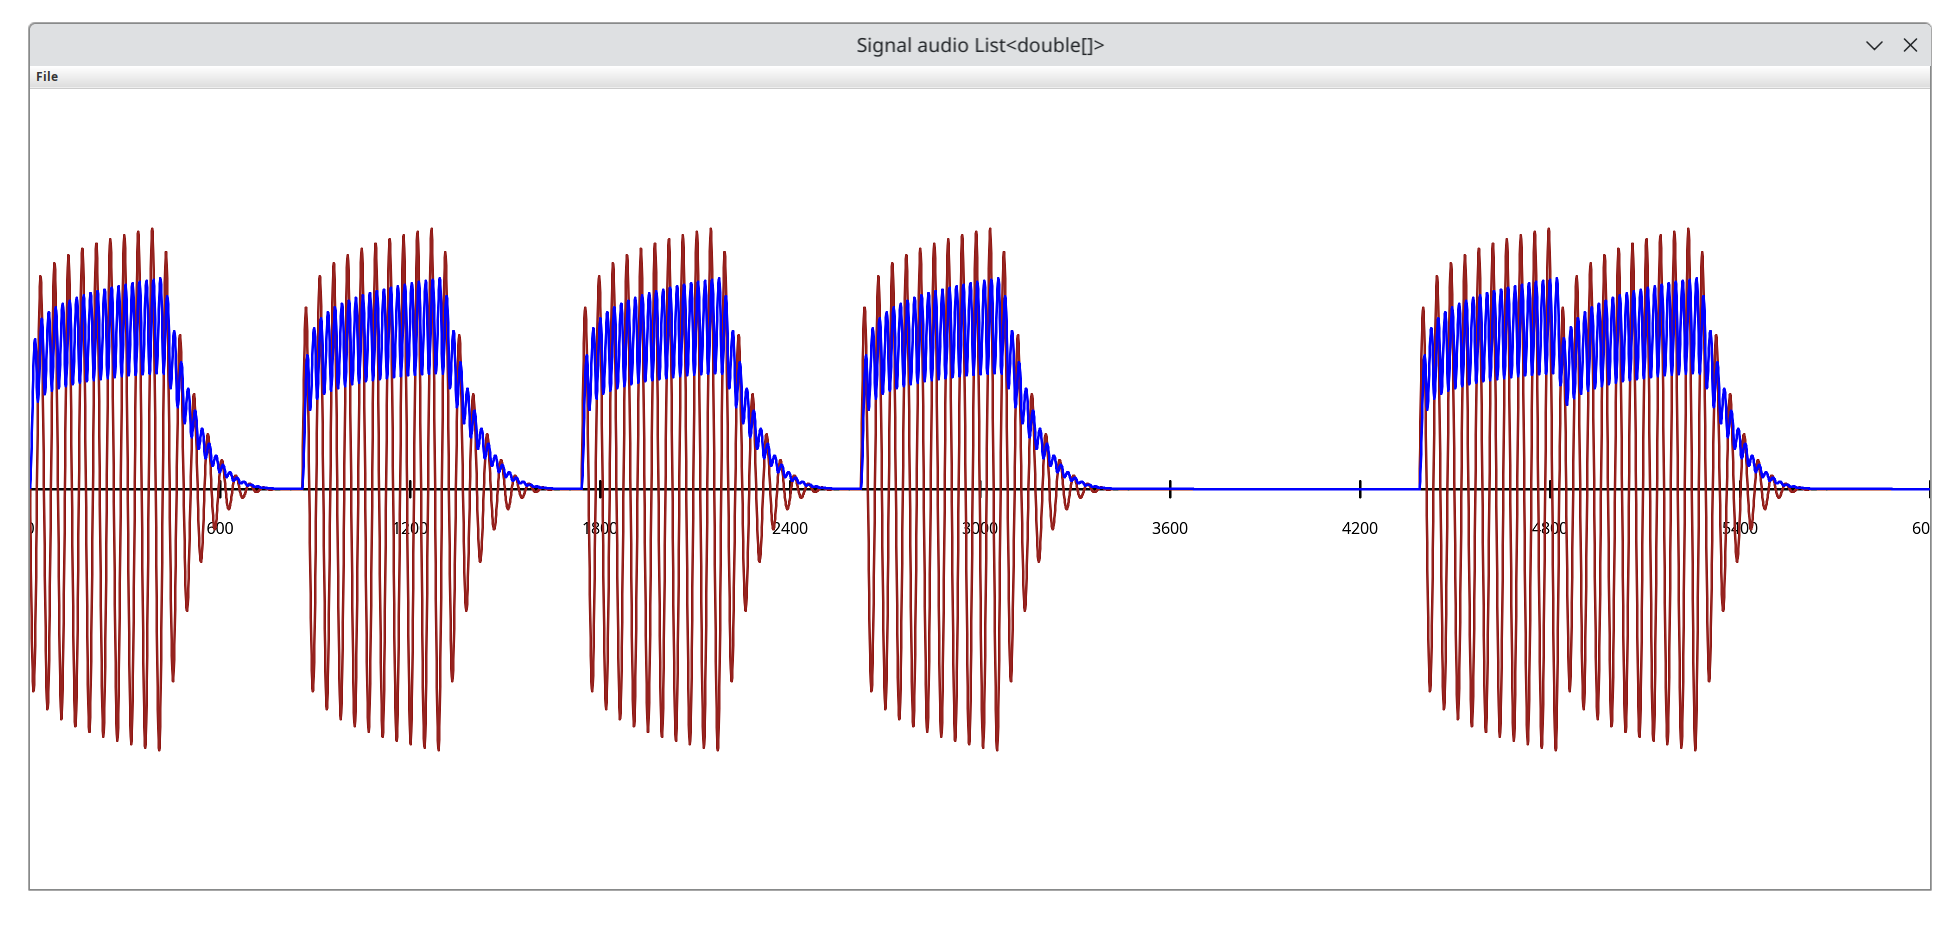
\includegraphics[width=15cm]{images/LP21000.png}
	\end{center}
	\caption{\textbf{EMA} Filter output in blue for a cut off frequency of \textbf{1kHz}}
\end{figure}

\begin{figure}[!h]
	\begin{center}
		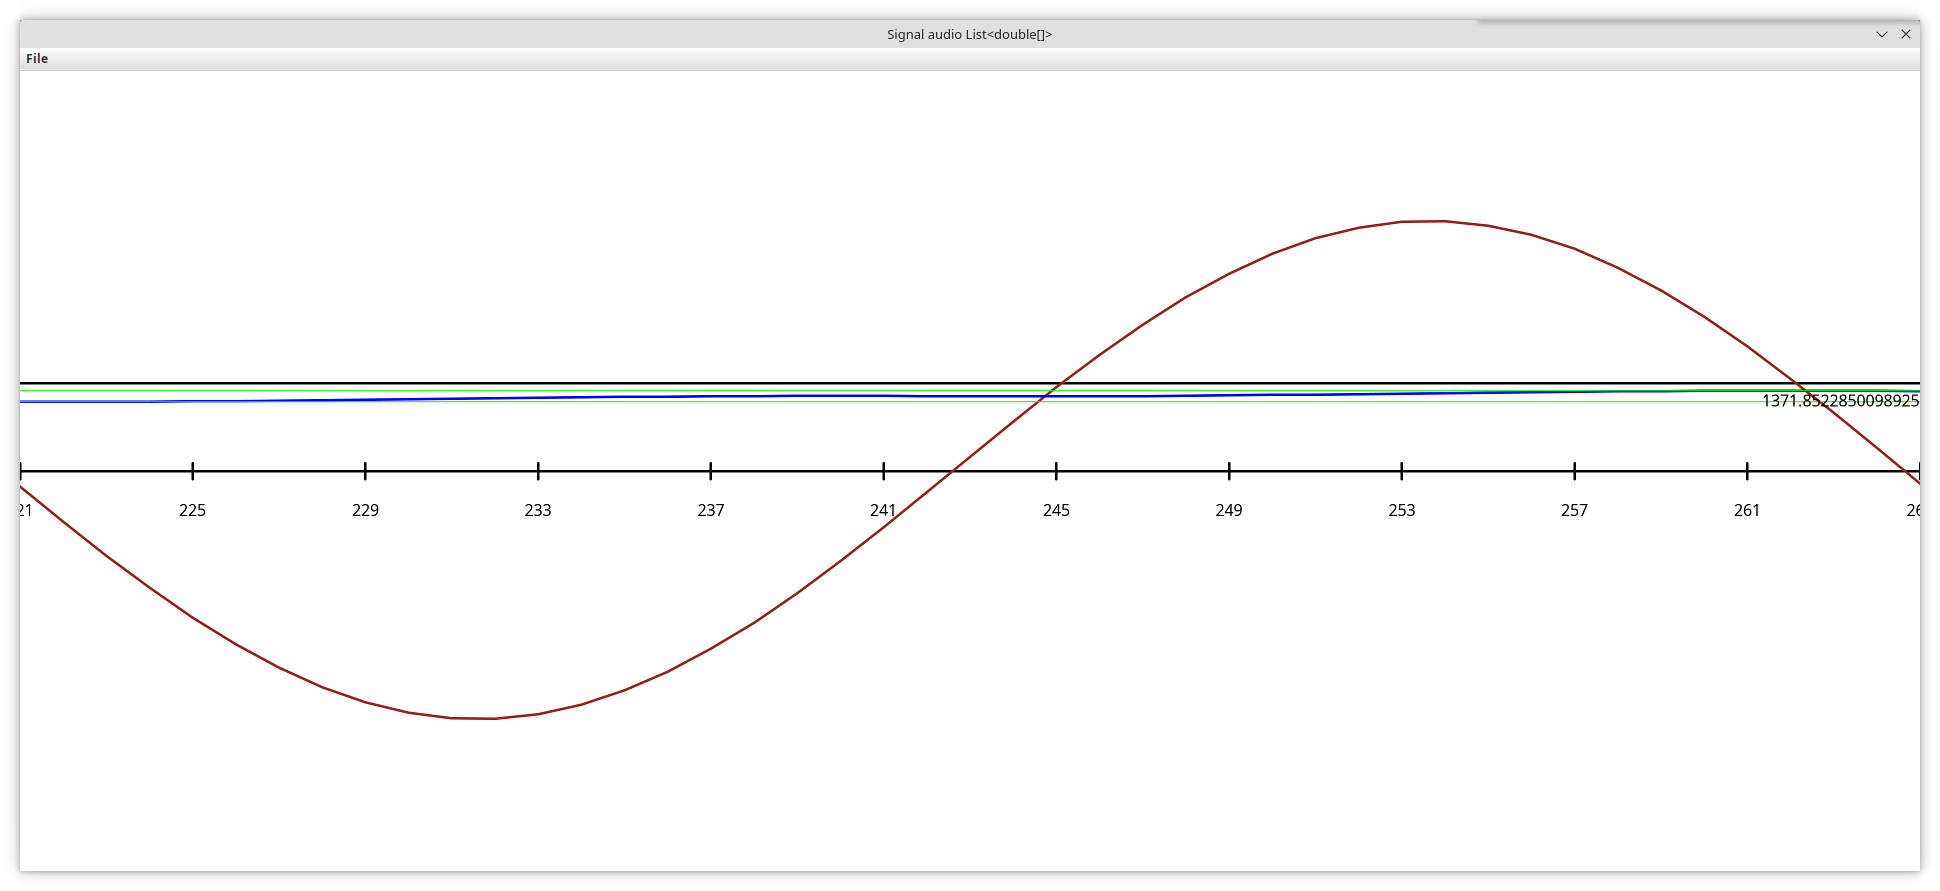
\includegraphics[width=15cm]{images/EMA20d1371.png}
	\end{center}
	\caption{\textbf{EMA} Delta of the signal amplitude for a cut off frequency value of 20Hz : 1371}
\end{figure}

\begin{figure}[!h]
	\begin{center}
		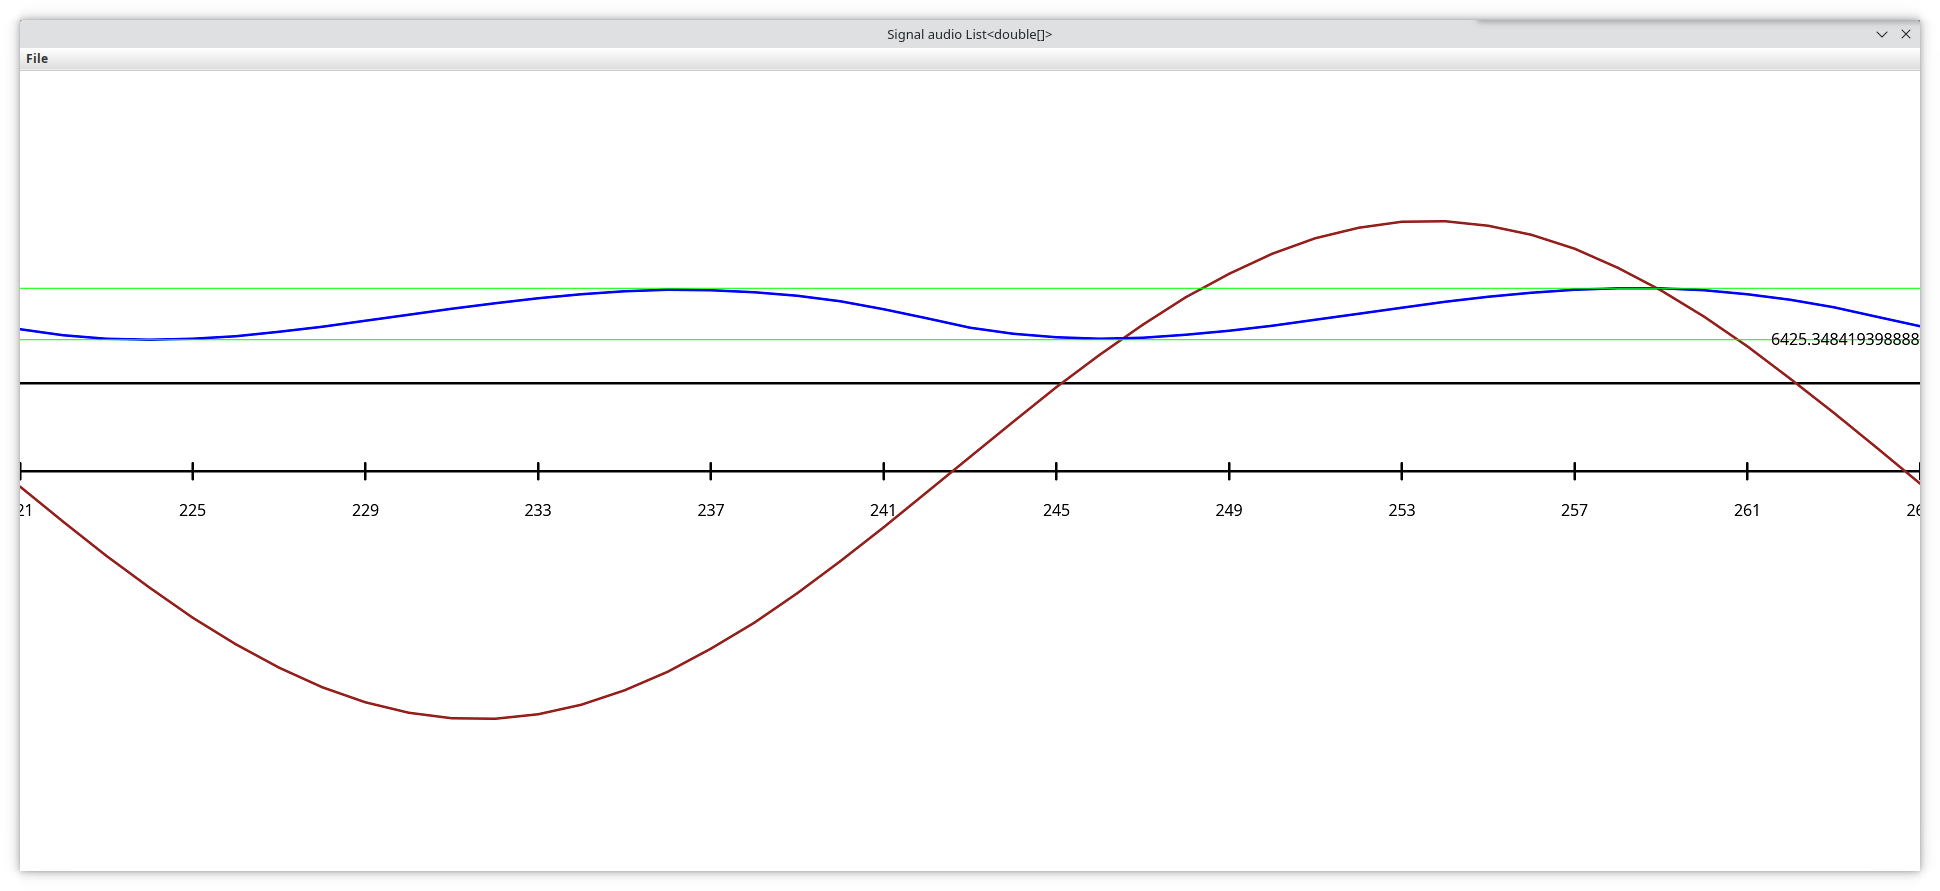
\includegraphics[width=15cm]{images/EMA500d6425.png}
	\end{center}
	\caption{\textbf{EMA} Delta of the signal amplitude for a cut off frequency value of 500Hz : 6425}
\end{figure}

\begin{figure}[!h]
	\begin{center}
		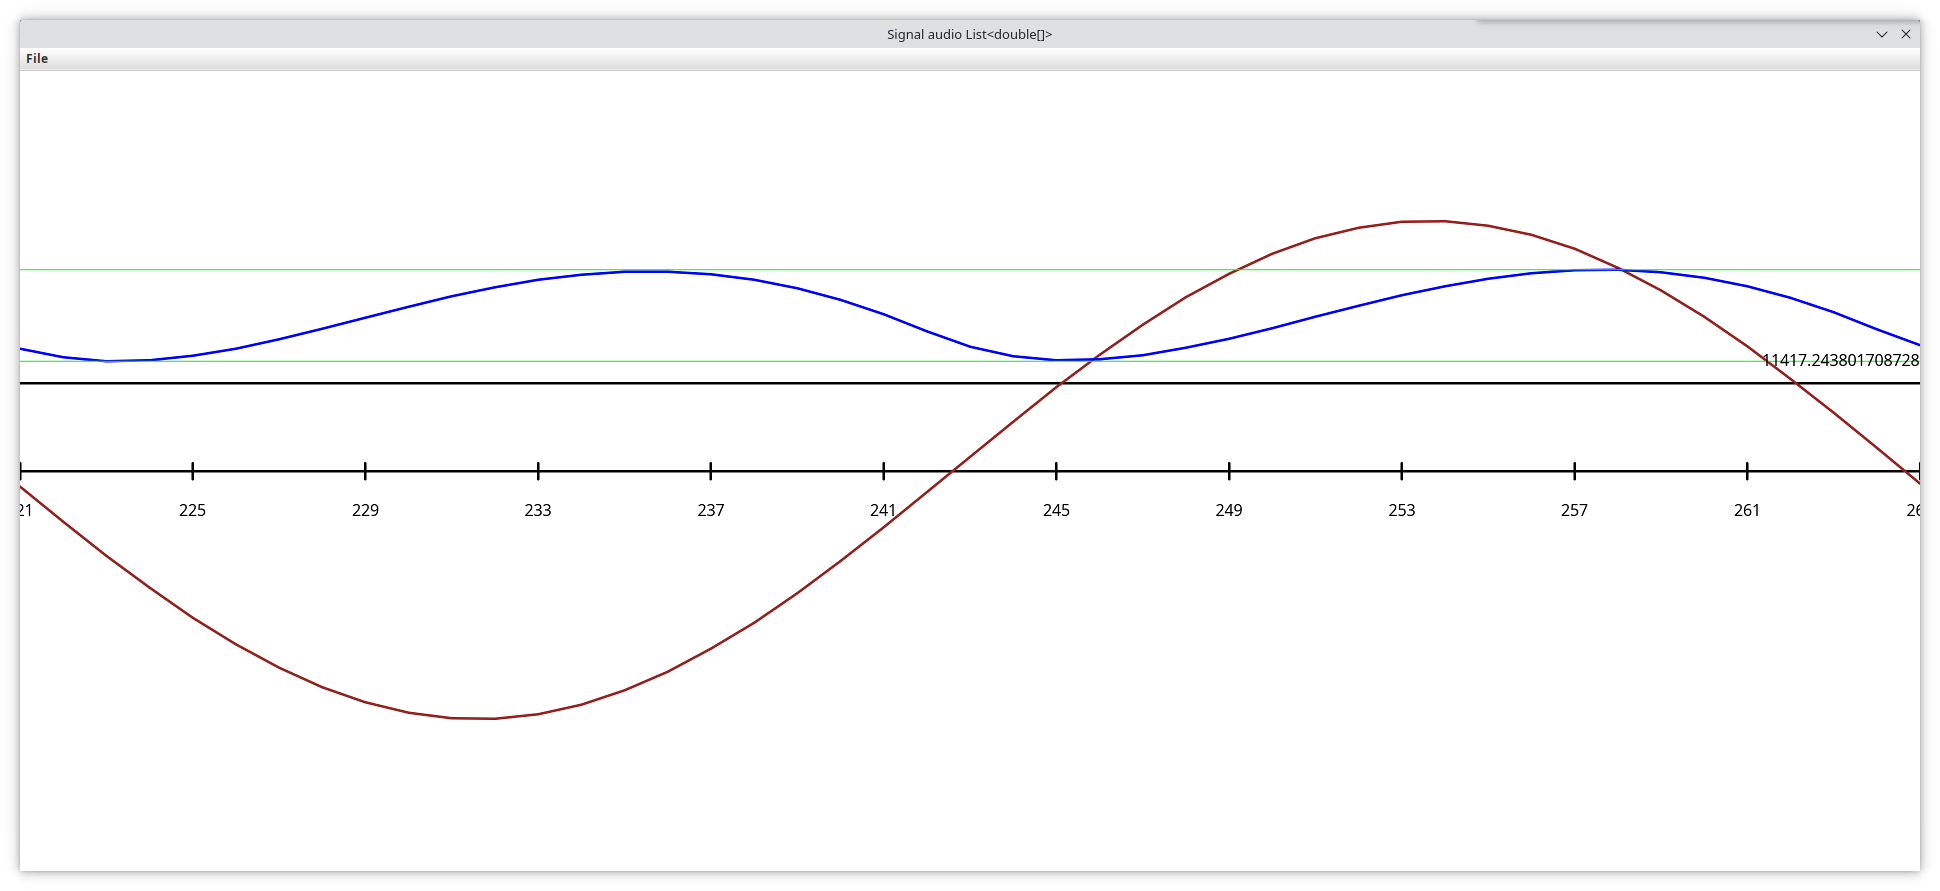
\includegraphics[width=15cm]{images/EMA1000d11417.png}
	\end{center}
	\caption{\textbf{EMA} Delta of the signal amplitude for a cut off frequency value of 1000Hz : 11417}
\end{figure}





\chapter{Discussion}

Both filters worked correctly for cut off values around 20 Hz making the delta between maximum and minimum amplitude for a period unoticable, going higher however increased that delta as seen by the signal oscillation being visible again, going above 1000Hz made the signal unreadable as it's amplitude was too fluctuent and needed a lower threshold that made noise be read as 1 instead of 0.

As both filters return the same kind of signal after processing a sinusoïd, it can be said that they are both usable for the same kind of work. It is important to note that the EMA filter offers a sharper frequency response rate as it drops and rise quicker than the SMA filter for a low cut off frequency. For a higher cut off frequency value, both filter seems to behave similarly keeping the shape of the original signal but with significant noise.

Performance wise the SMA filter is way behind the EMA Filter with processing getting longer as the number of samples it needs to filter the signal rises. On the other hand, the EMA filter is not impacted by the value for it's cut off frequency making it better than the SMA filter as the frequency of signal to process increases. This is reflected on the time it takes for a filter to process an increasingly bigger file. There is already an 11 ms difference for a file containing 13 characters but it goes up to a 2 seconds difference for a 6307 characters long file. An other way to interpret this data is to consider that it takes the SMA filter 4.27 ms of processing per character while the EMA filter hovers around 0.15 ms per character.
\chapter{Conclusion}

Looking at the data, there seems to be no benefits to using the SMA filter instead of an EMA filter to filter out the high frequencies of a sinousoïdal signal. The EMA filter is quicker and sharper than the SMA filter.

\newpage

%récupérer les citation avec "/footnotemark"
\nocite{*}



\end{document}